\section{Variational Autoencoders~--~VAEs}\label{VAEs}

Generative models, as defined in the seminal work by \citeauthor{diggleImplicitPrescribed}, fall into two primary categories: prescribed and implicit models. Prescribed models leverage well-formulated, often parametric, mathematical expressions for the probability density function (pdf), thus facilitating easier analytical interpretation of the distributions. Implicit models, on the other hand, synthesize new data samples without an explicit pdf, approximating the data distribution based on the training dataset \citep{diggleImplicitPrescribed}. Variational Autoencoders (VAEs) are aligned with the prescribed models category, given their reliance on an explicit formulation of the pdf to operate efficiently. This feature makes VAEs suitable for tasks that require not only the generation but also the understanding of complex data distributions \citep{kingmaVAE,rezendeVAE,GoodfellowDeepLearning}. In contrast, Generative Adversarial Networks (GANs) are a prime example of the implicit models category \citep{goodfellowGAN}.

VAEs are essentially based on the architecture of Autoencoders, which apply an iterative process to identify the optimal encoder and decoder pair, aiming to minimize the reconstruction loss while preserving substantial information after dimensionality reduction. The encoder compresses the input data into a low-dimensional representation, or ``code'' \citep{hintonCode, GoodfellowDeepLearning}, which captures the most relevant features of the input, within a latent space. The decoder then reconstructs the original input from this compressed latent vector, with the error between the output and original data being backpropagated to optimize the model’s weights \citep{GoodfellowDeepLearning, michelucci2022introduction}. Although this process balances data compression and information preservation, a drawback remains that if the encoder and decoder are too closely matched, the latent space becomes uncontrollable resulting in a lack of interpretability and regularity \citep{michelucci2022introduction}.

Autoencoders, in their essence, aim for approximate rather than perfect replication of the input data, which forces the model to prioritize certain aspects of the input to copy, often learning useful properties of the data \citep{GoodfellowDeepLearning}. This dimensionality reduction proves beneficial in enhancing classification tasks' efficiency by reducing computational costs and memory overhead, and improving information retrieval in low-dimensional spaces \citep{GoodfellowDeepLearning}. However, traditional autoencoders fall short in generating new data due to the unregulated nature of the latent spaces.

The challenge posed by unregulated latent spaces in autoencoders is great when generating new data. Attempting to decode a randomly selected point from this latent space often leads to unusable results because part of the latent space does not match any data point. Simply trying to organize the latent space proves difficult as its structure is affected by the distribution of the source space, the dimensionality of the latent space, and the architecture of the encoder \citep{michelucci2022introduction}.
In essence, traditional autoencoders are not designed to generate new data; their main function is to copy and reconstruct the given input \citep{GoodfellowDeepLearning}.

\begin{figure}[ht]
    \centering
      \hspace{.8cm}
      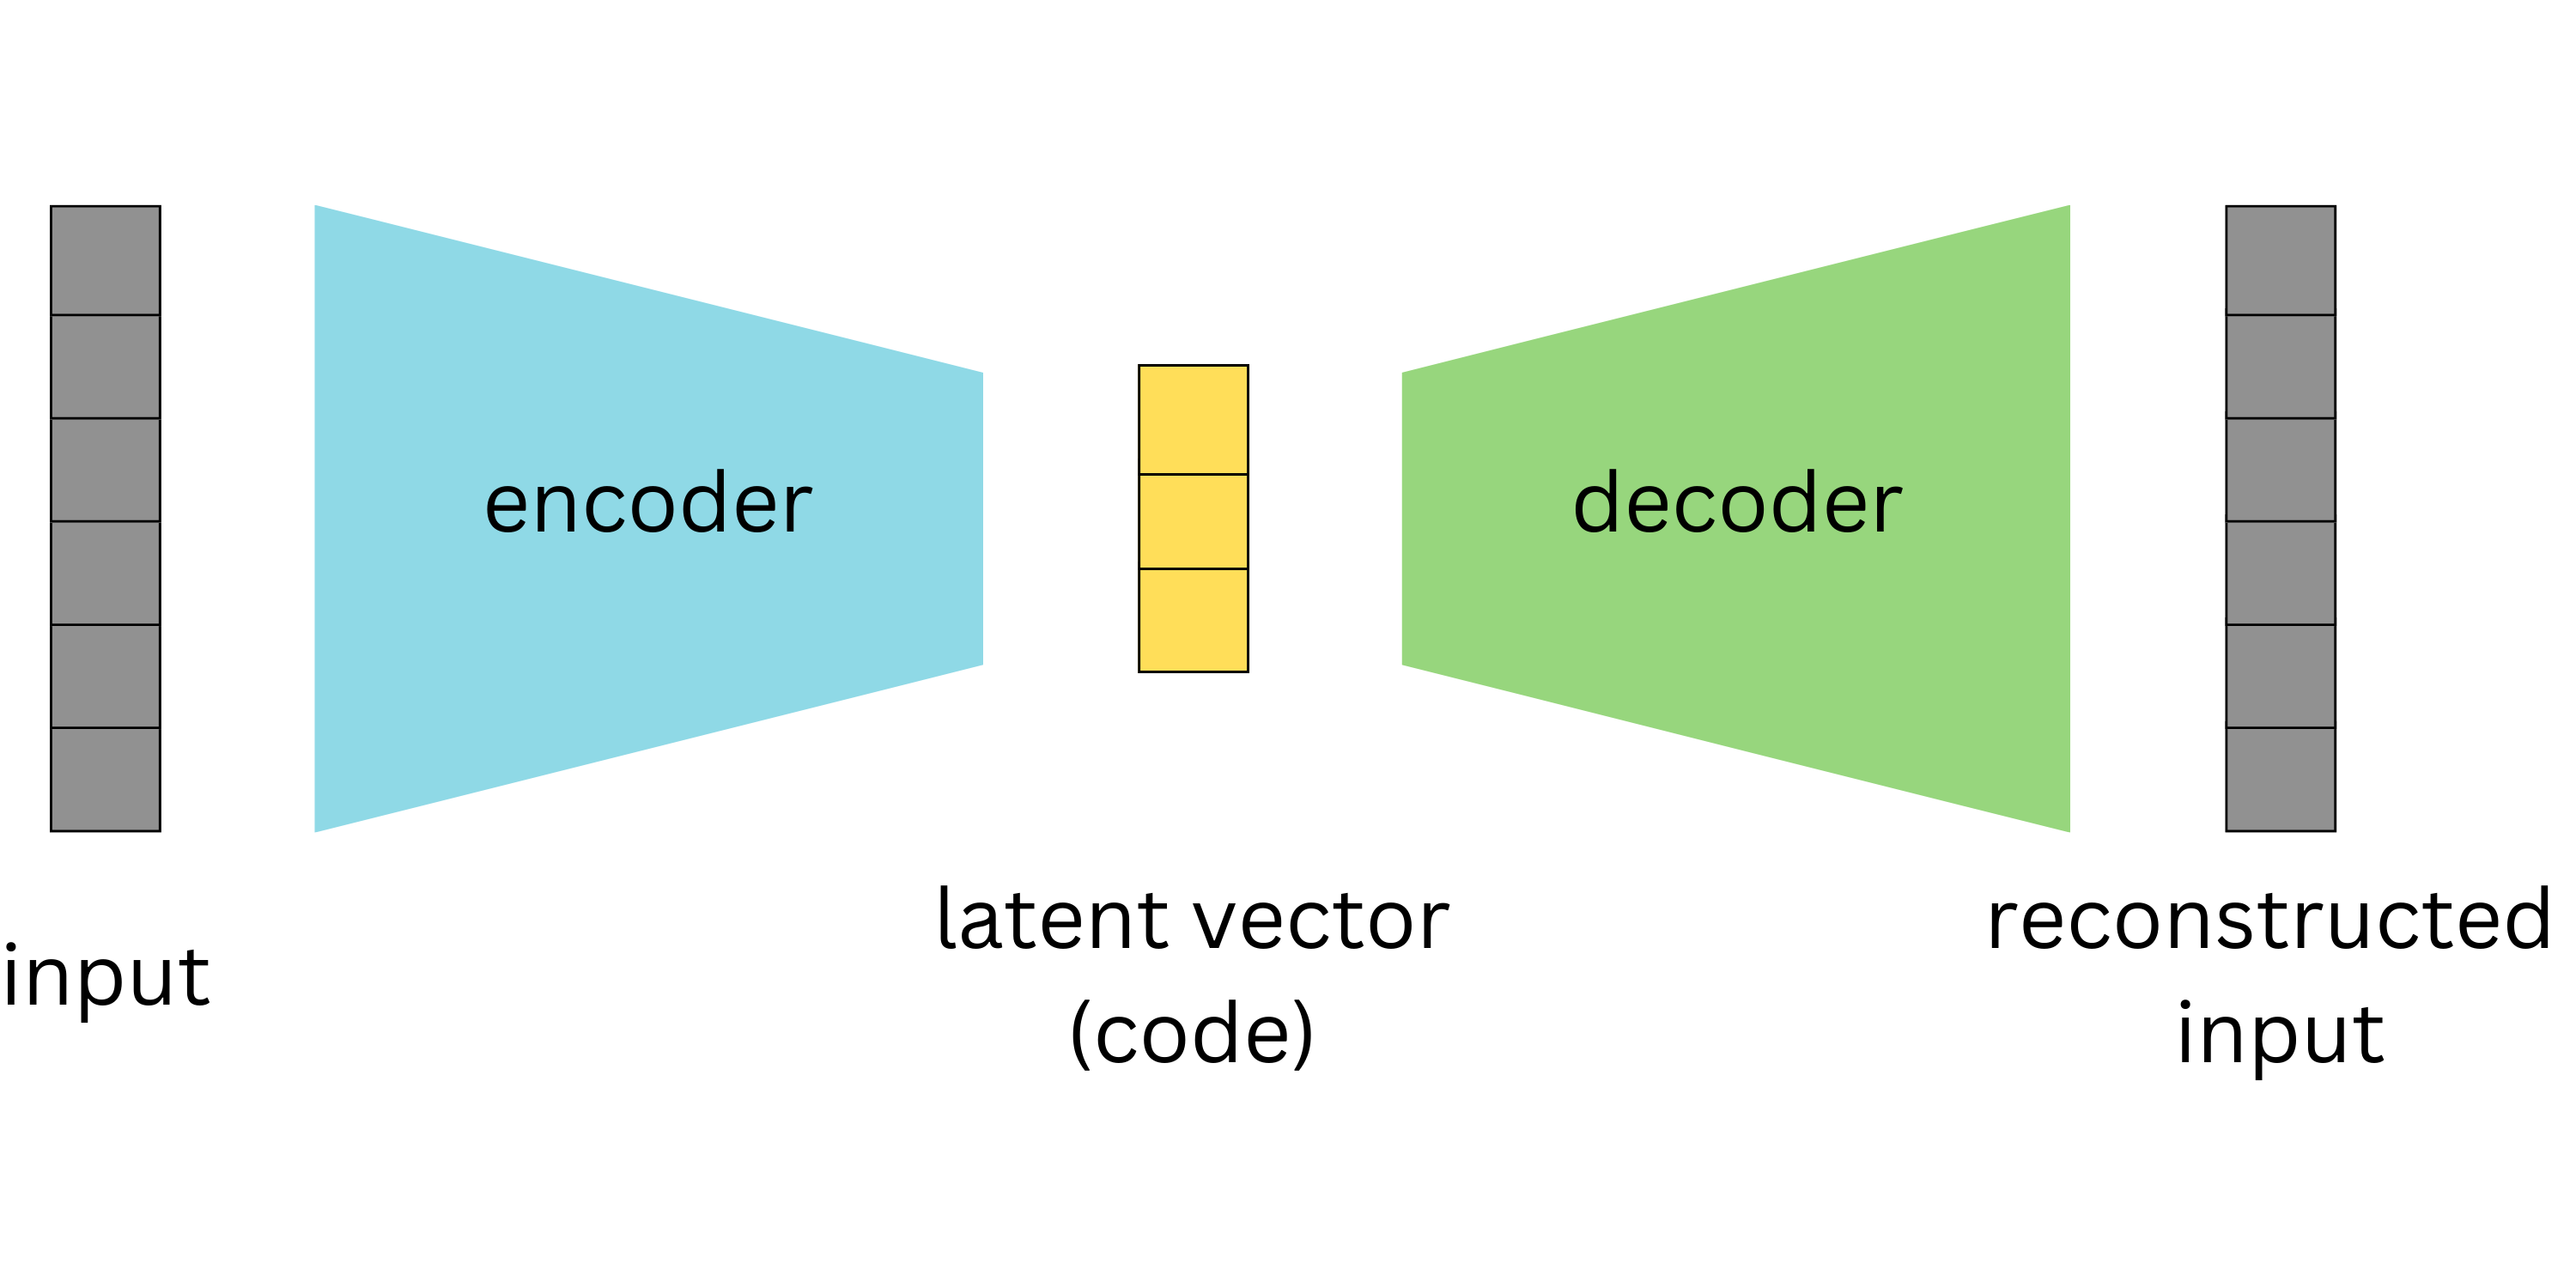
\includegraphics[width=.7\columnwidth]{figures/Autoencoder.png}
      \caption{Autoencoder: The encoder reduces the input dimension to a latent vector that captures the most important features. The decoder then uses this vector to reconstruct the input, with training aimed at minimizing reconstruction loss. TODO\@ ADD LOSS\@ https://towardsdatascience.com/difference-between-autoencoder-ae-and-variational-autoencoder-vae-ed7be1c038f2}\label{fig:figureAE}
\end{figure}

VAEs tackle the limitations of traditional autoencoders by implementing enhanced regularization of the latent space during training. Although the iterative process largely remains the same, VAEs deviate by encoding a distribution, shaped by the parameters \(\mu\) and \(\sigma\), over the latent space instead of a single point \citep{doerschVAE}. Then, a point is sampled from this distribution to represent the latent variable \(z\). This sampled point is used to calculate the reconstruction error, which is then backpropagated to update the model's weights.

A major objective of VAEs is to compute the data likelihood, \(P(X)\), through strategic sampling of latent variables \(z\). This computation is important because it follows the intuition of maximum likelihood, which states that ``if the model is likely to produce training set samples, then it is also likely to produce similar samples, and unlikely to produce dissimilar one'' \citep{doerschVAE}. Strategic sampling here means that the model uses a new function \(Q(z|X)\) that, given a value of X, returns a distribution over latent variables \(z\) that is most likely to have produced the data point \(X\) \citep{doerschVAE}. The core equation for VAEs is expressed as follows:

\[
\log P(X) - D_{KL} \left[ Q(z|X) \parallel P(z|X) \right] = \mathbb{E}_{z \sim Q} \left[ \log P(X|z) \right] - D_{KL} \left[ Q(z|X) \parallel P(z) \right]
\]

~\citep{doerschVAE}.
This equation first aims to maximize the log likelihood of the data, denoted as \(\log P(X)\). A higher log likelihood means that the model is good at recreating data. The KL divergence term \(D_{KL} \) acts as an error term, ensuring that \(Q(z|X)\) accurately reproduces the posterior distribution \(P(z|X)\) \citep{doerschVAE}. By minimizing the divergence of \(P\) and \(Q\), it is ensured that \(Q\) closely resembles \(P\). On the right hand side, the first part determines the expected log-likelihood of the reconstruction data given the latent variables \(z\), under the distribution \(Q\). The KL divergence between the posterior \(Q(z|X)\) and the prior distribution \(P(z)\), helps to regularize \(Q\). This side of the equation can be optimized using stochastic gradient descent with a suitable choice of \(Q\) \citep{doerschVAE}. 

\begin{figure}[ht]
    \centering
      \hspace{.8cm}
      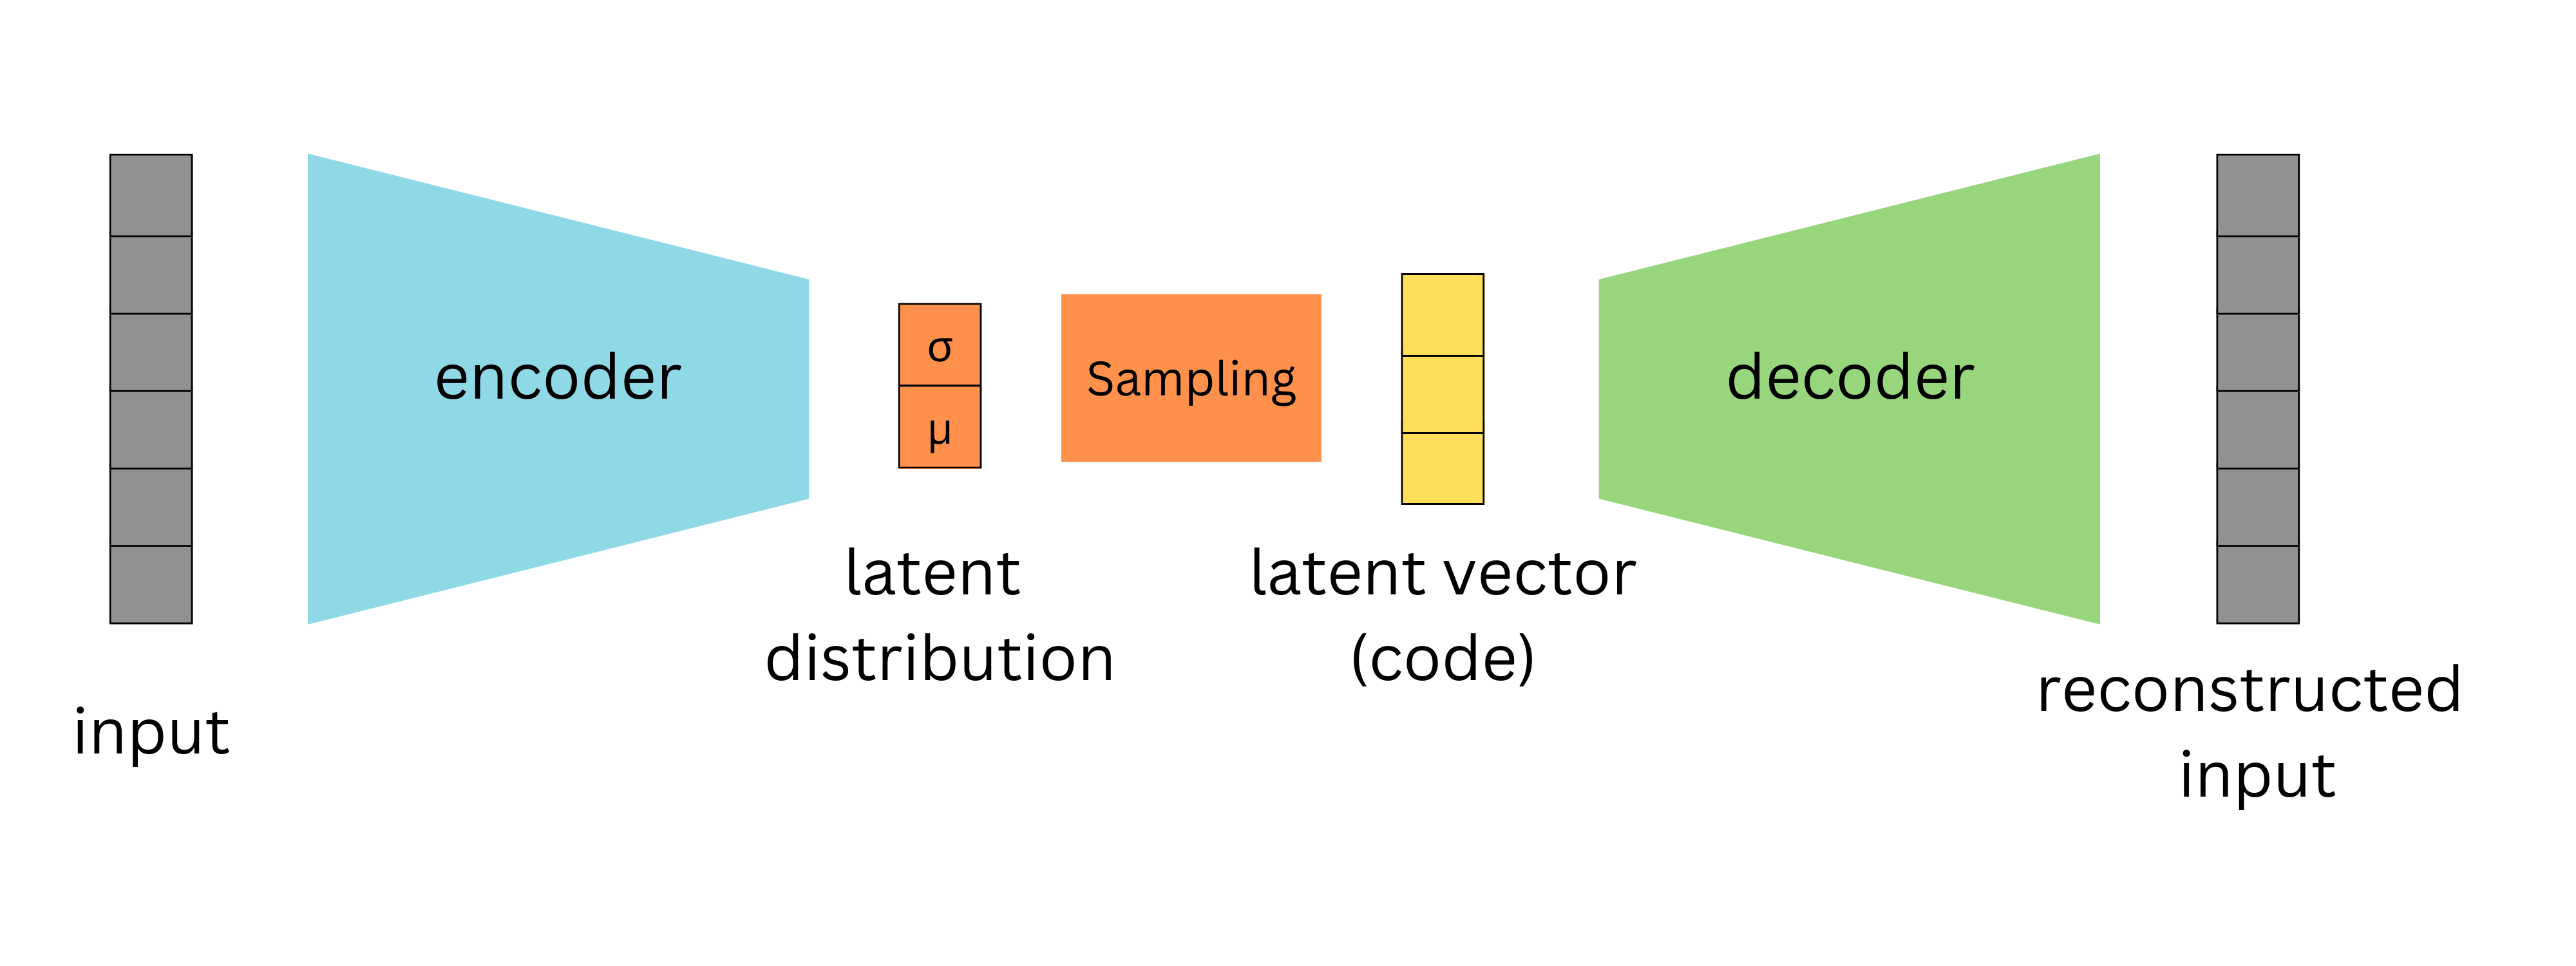
\includegraphics[width=.9\columnwidth]{figures/VAE.png}
      \caption{Functionality of a Variational Autoencoder, demonstrating incorporation of the latent distribution~--~the mean and standard deviation~--~for enhancing latent space regularization.}\label{fig:figureVAE}
\end{figure}

Despite their capabilities, VAEs exhibit some limitations. According to \citeauthor{GoodfellowDeepLearning}, the generated samples can often be blurry. The reason for this is not fully 
understood, but the blurriness observed may be due to their optimization process, which minimizes Kullback-Leibler divergence. This could lead the model to assign high probabilities to ``points that occur in the training set, but may also assign high probability to other points [\(\ldots\)] which may include blurry images'' \citep{GoodfellowDeepLearning}. The Gaussian distribution often used in VAEs for the generative model may also contribute to this effect, as it can ignore minor features in the input data \citep{GoodfellowDeepLearning}. Another issue is that VAEs typically utilize only a small portion of the latent space, which might further compromise the quality of generated images \citep{GoodfellowDeepLearning}. The performance of the model is also sensitive to the choice of priors for the latent space, making hyperparameter tuning an essential aspect of working with VAEs \citep{kingmaVAE, higginsVAE}. 

